No desenvolvimento se detalha a pesquisa ou estudo realizado. É a parte mais
extensa da monografia. É no desenvolvimento que encontraremos a fundamentação
teórica, a metodologia, os resultados e a discussão.

Levando-se em consideração sobre estudos em acessibilidade em documentos
digitais, a escolha da fonte é uma decisão importante, pois é um elemento
imprescindível na monografia. Deve-se dar preferências as fontes sem serifa,
que são indicadas para leitura de documentos mais compreensível em word e PDF.

De acordo com Salton, Agnol e Turcatti (2017, p.~61),

\begin{citacaolonga}
É recomendada a utilização de fontes sem serifa (sans-serif), como Arial e
Verdana, uma vez que fontes serifadas podem dificultar a leitura de alguns
grupos de usuários, já que dão a impressão de estarem unidas devido aos
prolongamentos nos fins das hastes das letras. Da mesma forma, recomenda-se
evitar o uso de fontes muito elaboradas, decoradas e cursivas, que podem
confundir usuários com baixa visão e dificultar a leitura de pessoas com
dificuldades de aprendizagem.
\end{citacaolonga}

Segundo Brasil (2010, p.~17),

\begin{citacaolonga}
Fontes serifadas dão a impressão de estarem unidas, devido aos prolongamentos
no fim das hastes das letras, podendo confundir usuários com baixa visão. Além
disso, fontes muito ``enfeitadas'' dificultam a leitura de pessoas com
dificuldade de aprendizagem.
\end{citacaolonga}

As fontes sem serifa (\textit{Sans Serif}) são mais limpa como, por exemplo, a
fonte Arial. As fontes serifadas possuem um prolongamento no final das hastes
das letras que podem confundir os leitores de baixa visão, como por exemplo,
Times New Roman e Courier New.

O tipo de fonte para trabalhos acadêmicos não é especificada nas normas da
ABNT, mas as fontes indicadas e mais utilizadas são a Arial e a Times New
Roman, pois a diferença entre ambas é muito pouca.

\textopadrao

\textopadrao

\section{Seção Secundária}

A seção secundária é uma subdivisão do texto a partir de uma seção primária.
Para a elaboração das seções primárias, secundárias, terciárias, quaternárias
e quinárias, a autor deve seguir as orientações da ABNT NBR 6024 que trata
sobre a numeração progressiva. Esta norma destaca gradualmente os títulos das
seções e orienta na utilização dos recursos de negrito, itálico ou sublinhado
e outros. As seções que estão no sumário devem estar idênticas às seções que
estão no texto (ABNT, 2012).

As tabelas são formas não discursivas de apresentarem informações das quais o
dado numérico se destaca como informação central (tabela~\ref{tab:ibge}). A
formatação das tabelas segue as orientações do Instituto Brasileiro de
Geografia e Estatística (IBGE).

\vspace{15pt}
\begin{table}[H]
  \caption{Estudantes de curso superior de graduação, por tipo de curso superior de\\
    graduação que frequentavam, segundo as classes de rendimento mensal\\
    domiciliar e de rendimento mensal domiciliar per capita - Brasil -- 2014}
  \label{tab:ibge}
  \tabelaibge\raggedright
  \setlength{\tabcolsep}{0pt}\renewcommand{\arraystretch}{1}\setlength{\arrayrulewidth}{0.5pt}
  \noindent\hspace*{-0.7pt}\begin{tabular}{@{}p{139.8pt}*{6}{p{56.06pt}}@{}}
    \hline
    \multirow{4}{139.8pt}[-26pt]{\centering Classes de rendimento mensal domiciliar e de
      rendimento mensal domiciliar \textit{per capita}}
      & \multicolumn{6}{|c}{\rule[-6.2pt]{0pt}{15pt}Estudantes de curso superior de graduação} \\ \cline{2-7}
      & \multicolumn{3}{|c|}{\rule[-4.5pt]{0pt}{15pt}Valores absolutos (1\hspace{1.7pt}000 pessoas)}
      & \multicolumn{3}{c}{Valores relativos (\%)} \\ \cline{2-7}
      & \multicolumn{1}{|c|}{\multirow{2}{*}[-11pt]{\centering Total}}
      & \multicolumn{2}{c|}{\rule[-12pt]{0pt}{30pt}\begin{tabular}[c]{@{}c@{}}Tipo de curso superior de graduação\\ que frequentavam\end{tabular}}
      & \multicolumn{1}{c|}{\multirow{2}{*}[-11pt]{\centering Total}}
      & \multicolumn{2}{c}{\begin{tabular}[c]{@{}c@{}}Tipo de curso superior de graduação\\ que frequentavam\end{tabular}} \\ \cline{3-4}\cline{6-7}
      & \multicolumn{1}{|c|}{}
      & \multicolumn{1}{c|}{\rule[-12pt]{0pt}{30pt}\begin{tabular}[c]{@{}c@{}}Era superior de\\ tecnologia\end{tabular}}
      & \multicolumn{1}{c|}{\begin{tabular}[c]{@{}c@{}}Não era superior\\ de tecnologia\end{tabular}}
      & \multicolumn{1}{c|}{}
      & \multicolumn{1}{c|}{\begin{tabular}[c]{@{}c@{}}Era superior de\\ tecnologia\end{tabular}}
      & \multicolumn{1}{c}{\begin{tabular}[c]{@{}c@{}}Não era superior\\ de tecnologia\end{tabular}} \\ \hline
    \rule[-2.7pt]{0pt}{15pt}\hfill\textbf{Total}\hfill\null & \nc{7\hspace{1.7pt}242} & \nc{477} & \nc{6\hspace{1.7pt}765} & \nc{100,0} & \nc{100,0} & \nc{100,0} \\[9pt]
    \rule[-2.7pt]{0pt}{15pt}\hspace{3.7pt}\textbf{Classes de rendimento mensal domiciliar} & & & & & & \\
    \rule[-2.7pt]{0pt}{15pt}\hspace{10.7pt}Sem rendimento a 1 salário mínimo (1) & \nc{188} & \nc{11} & \nc{177} & \nc{2,6} & \nc{2,3} & \nc{2,6} \\
    \rule[-2.7pt]{0pt}{15pt}\hspace{10.7pt}Mais de 1 a 2 salários mínimos & \nc{612} & \nc{31} & \nc{581} & \nc{8,4} & \nc{6,5} & \nc{8,6} \\
    \rule[-2.7pt]{0pt}{15pt}\hspace{10.7pt}Mais de 2 a 3 salários mínimos & \nc{860} & \nc{51} & \nc{809} & \nc{11,9} & \nc{10,8} & \nc{12,0} \\
    \rule[-2.7pt]{0pt}{15pt}\hspace{10.7pt}Mais de 3 a 5 salários mínimos & \nc{1\hspace{1.7pt}664} & \nc{116} & \nc{1\hspace{1.7pt}547} & \nc{23,0} & \nc{24,4} & \nc{22,9} \\
    \rule[-2.7pt]{0pt}{15pt}\hspace{10.7pt}Mais de 5 a 10 salários mínimos & \nc{2\hspace{1.7pt}286} & \nc{166} & \nc{2\hspace{1.7pt}121} & \nc{31,6} & \nc{34,8} & \nc{31,3} \\
    \rule[-2.7pt]{0pt}{15pt}\hspace{10.7pt}Mais de 10 a 20 salários mínimos & \nc{914} & \nc{60} & \nc{854} & \nc{12,6} & \nc{12,6} & \nc{12,6} \\
    \rule[-2.7pt]{0pt}{15pt}\hspace{10.7pt}Mais de 20 salários mínimos & \nc{357} & \nc{15} & \nc{342} & \nc{4,9} & \nc{3,1} & \nc{5,1} \\
    \rule[-2.7pt]{0pt}{15pt}\hspace{10.7pt}Sem declaração & \nc{360} & \nc{26} & \nc{334} & \nc{5,0} & \nc{5,5} & \nc{4,9} \\
    \hline
  \end{tabular}\par
  \fonte[5.7pt]{IBGE (2014)}
\end{table}

\textopadrao

\textopadrao

\subsection{Seção Terciária}

A seção terciária é uma subdivisão do texto a partir de uma seção secundária.
Para a elaboração das seções primárias, secundárias, terciárias, quaternárias
e quinárias, a autor deve seguir as orientações da ABNT NBR 6024 que trata
sobre a numeração progressiva. Esta norma destaca gradualmente os títulos das
seções e orienta na utilização dos recursos de negrito, itálico ou sublinhado
e outros. As seções que estão no sumário devem estar idênticas às seções que
estão no texto (ABNT, 2012).

São consideradas ilustrações: os desenhos, esquema, fluxograma, fotografia,
gráfico, mapa, organograma, planta, quadro, retrato, figura, imagem, entre
outros. A identificação da ilustração é inserida na parte superior seguida de
seu número de ordem que se sucede dentro do texto, em algarismos arábicos,
travessão e do respectivo título. Na parte inferior da ilustração deve-se
colocar a fonte consultada. Caso necessite, após a fonte pode colocar legenda,
notas e outras informações. Deve-se citar no texto e inserir o mais próximo do
trecho a que se refere (ABNT, 2012).

Como exemplo, segue a figura~\ref{fig:1} abaixo.

\begin{figure}[H]
  \caption{Níveis do curso de Biblioteconomia na Biblioteca Nacional}
  \label{fig:1}
  \centering
  \begin{minipage}{225.6pt}
    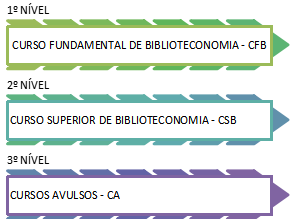
\includegraphics[width=225.6pt]{figuras/niveis-biblioteconomia.png}\par
    \fonte[4pt]{Elaborado pelos autores (2021).}
  \end{minipage}
\end{figure}

\textopadrao

\textopadrao

\subsubsection{Seção Quartenária}

A seção quaternária é uma subdivisão do texto a partir de uma seção terciária.
Para a elaboração das seções primárias, secundárias, terciárias, quaternárias
e quinárias, a autor deve seguir as orientações da ABNT NBR 6024 que trata
sobre a numeração progressiva. Esta norma destaca gradualmente os títulos das
seções e orienta na utilização dos recursos de negrito, itálico ou sublinhado
e outros. As seções que estão no sumário devem estar idênticas às seções que
estão no texto (ABNT, 2012).

\textopadrao

\textopadrao

\paragraph{Seção Quinária}

A seção quinária é uma subdivisão do texto a partir de uma seção quartenária.
Para a elaboração das seções primárias, secundárias, terciárias, quaternárias
e quinárias, a autor deve seguir as orientações da ABNT NBR 6024 que trata
sobre a numeração progressiva. Esta norma destaca gradualmente os títulos das
seções e orienta na utilização dos recursos de negrito, itálico ou sublinhado
e outros. As seções que estão no sumário devem estar idênticas às seções que
estão no texto (ABNT, 2012).

Os quadros possuem a mesma forma de apresentação das ilustrações. De forma
geral apresentam informações textuais, conforme o quadro~\ref{qua:normas}.

\vspace{3pt}
\begin{quadro}[H]
  \caption{Normas utilizadas na elaboração de um trabalho acadêmico}
  \label{qua:normas}
  \quadrotexto\raggedright
  \setlength{\tabcolsep}{5pt}\setlength{\arrayrulewidth}{0.5pt}
  \noindent\hspace*{20.9pt}\begin{tabular}{|>{\raggedright}p{39.6pt}|>{\raggedright}p{318.6pt}|>{\centering\arraybackslash}p{30.9pt}|}
    \hline
    \multicolumn{1}{|c|}{\textbf{Autor}} & \multicolumn{1}{c|}{\textbf{Título}} & \textbf{Ano} \\ \hline
    ABNT & NBR 6023, Informação e documentação -- Referências -- Elaboração. & 2018 \\ \hline
    ABNT & NBR 6024, Informação e documentação -- Numeração progressiva das seções de um documento escrito -- Apresentação. & 2012 \\ \hline
    ABNT & NBR 6027, Informação e documentação -- Sumário -- Apresentação. & 2012 \\ \hline
    ABNT & NBR 6028, Informação e documentação -- Resumo -- Procedimento. & 2021 \\ \hline
    ABNT & NBR 6034, Informação e documentação -- Índice -- Apresentação. & 2004 \\ \hline
    ABNT & NBR 10520, Informação e documentação -- Citações em documentos -- Apresentação. & 2023 \\ \hline
    IBGE & Normas de apresentação tabular & 1993 \\ \hline
  \end{tabular}\par
  \fonte[22.9pt]{Elaborado pelo autor (2021).}
\end{quadro}

\textopadrao

\textopadrao

\section{Seção Secundária}

A seção secundária é uma subdivisão do texto a partir de uma seção primária.
Para a elaboração das seções primárias, secundárias, terciárias, quaternárias
e quinárias, a autor deve seguir as orientações da ABNT NBR 6024 que trata
sobre a numeração progressiva. Esta norma destaca gradualmente os títulos das
seções e orienta na utilização dos recursos de negrito, itálico ou sublinhado
e outros. As seções que estão no sumário devem estar idênticas às seções que
estão no texto (ABNT, 2012).

\textopadrao

\textopadrao

\subsection{Seção Terciária}

A seção terciária é uma subdivisão do texto a partir de uma seção secundária.
Para a elaboração das seções primárias, secundárias, terciárias, quaternárias
e quinárias, a autor deve seguir as orientações da ABNT NBR 6024 que trata
sobre a numeração progressiva. Esta norma destaca gradualmente os títulos das
seções e orienta na utilização dos recursos de negrito, itálico ou sublinhado
e outros. As seções que estão no sumário devem estar idênticas às seções que
estão no texto (ABNT, 2012).

\textopadrao

\textopadrao

\subsubsection{Seção Quartenária}

A seção quaternária é uma subdivisão do texto a partir de uma seção terciária.
Para a elaboração das seções primárias, secundárias, terciárias, quaternárias
e quinárias, a autor deve seguir as orientações da ABNT NBR 6024 que trata
sobre a numeração progressiva. Esta norma destaca gradualmente os títulos das
seções e orienta na utilização dos recursos de negrito, itálico ou sublinhado
e outros. As seções que estão no sumário devem estar idênticas às seções que
estão no texto (ABNT, 2012).

\textopadrao

\textopadrao

\paragraph{Seção Quinária}

A seção quinária é uma subdivisão do texto a partir de uma seção quartenária.
Para a elaboração das seções primárias, secundárias, terciárias, quaternárias
e quinárias, a autor deve seguir as orientações da ABNT NBR 6024 que trata
sobre a numeração progressiva. Esta norma destaca gradualmente os títulos das
seções e orienta na utilização dos recursos de negrito, itálico ou sublinhado
e outros. As seções que estão no sumário devem estar idênticas às seções que
estão no texto (ABNT, 2012).

\textopadrao

\textopadrao
